\chapter{Interactive Genetic Algorithm for Parameter Optimisation}
\label{Chapter4}

Building upon our distance-based approach for natural terrain transitions presented in Chapter \ref{Chapter3}, we now address the parameter optimisation challenge detailed in Section \ref{parameter_optimization}. As established in Section \ref{parameter_space_challenge}, the complexity of parameter tuning in procedural terrain generation creates significant barriers to practical adoption, particularly when multiple algorithms are combined in complex pipelines.

In this chapter, we present our specific implementation of an Interactive Genetic Algorithm (IGA) for parameter optimisation and ordering of terrain operations in constrained terrain generation. Drawing directly from the foundational work of \textcite{Walsh10} discussed in Section \ref{interactive_genetic_algorithms}, we have adapted and extended their approach to address the unique challenges of our constrained terrain generation system. Our implementation transforms parameter tuning from a technical optimisation problem into an intuitive process of guided aesthetic selection, making advanced terrain generation accessible to both technical and non-technical users.

\section{Adaptation of IGA for Constrained Terrain Generation}

Interactive Genetic Algorithms provide a powerful framework for navigating complex parameter spaces through human-guided evolution. However, applying IGA to constrained terrain generation presents unique challenges that require careful adaptation of the basic IGA framework.

The fundamental challenge lies in the intersection of two complex problem domains: the inherent parameter space complexity of procedural terrain generation and the additional constraints introduced by our distance-based approach for handling fixed height areas. This intersection creates a parameter optimisation problem that is both computationally demanding and aesthetically nuanced.

\subsection{Parameter Space Complexity in Our System}

The parameter space complexity problem becomes particularly acute in our constrained terrain generation system. Our pipeline combines multiple algorithmic components, each with its own parameter set, that must work harmoniously to produce natural-looking terrain around fixed constraints. Unlike simpler terrain generation systems that might rely on a single algorithm with a handful of parameters, our approach requires managing multiple interdependent operations.

In our specific implementation, a typical terrain might include operations such as Perlin noise generation (frequency, octaves, persistence, amplitude), Voronoi-based mountain generation (peak count, falloff rate, height ranges), distance-based smoothing operations (iteration counts, strength parameters), and erosion simulations (threshold values, erosion rates). The interdependency between these parameters, combined with the additional complexity introduced by our distance-based constraint handling, creates a parameter space that resists systematic exploration through traditional manual tuning approaches.

Consider, for example, how adjusting the amplitude of Perlin noise affects not only the overall terrain but also the effectiveness of subsequent distance-based smoothing operations. A terrain with higher amplitude variations may require more aggressive smoothing near constraint boundaries, which in turn affects the natural appearance of transitions. These parameter dependencies make manual tuning increasingly impractical as the system grows in sophistication.

\subsection{From Theory to Implementation: Addressing Previous Limitations}

Our implementation directly addresses the fundamental limitation identified by \textcite{Walsh10}: the difficulty of defining mathematical fitness functions for inherently subjective terrain quality. While their pioneering work demonstrated the feasibility of using human judgment in terrain evolution, their approach was constrained by fixed-length binary encodings that could only represent a limited parameter space.

We extend their approach in several critical ways to address the specific requirements of constrained generation and adapt it to our system. These challenges, combined with the constraint-specific modifications we introduce in our distance-based approach, make traditional parameter optimisation approaches impractical. As discussed in Section \ref{interactive_genetic_algorithms}, Interactive Genetic Algorithms provide an elegant solution by leveraging human aesthetic judgment while automating the technical aspects of parameter space exploration.

Our implementation builds directly upon the terrain generation IGA approach pioneered by \textcite{Walsh10}, but extends it in several critical ways:

\textbf{Variable-Length Genome Representation}: Unlike the fixed-length binary encoding of an individual used by \textcite{Walsh10}, our system employs flexible, operation-based individuals(genomes) that can represent varying numbers and types of terrain operations. This allows the evolution of not just parameter values but also the structure and complexity of terrain generation pipelines themselves.

\textbf{Domain-Specific Genetic Operators}: We implement specialised crossover and mutation operations designed specifically for terrain generation pipelines, incorporating domain knowledge about effective operation sequences. Rather than generic mutations, our operators understand the semantic meaning of terrain operations and can make intelligent modifications.

\textbf{Constraint-Aware Evaluation}: Our preview generation and evolution process explicitly account for fixed height constraints, ensuring that evolved solutions respect the constraint boundaries established in our distance-based approach. This integration ensures that the IGA explores only feasible solutions that can work within the constraint framework.

\subsection{Integration with Distance-Based Constraint Handling}

The integration of IGA with our distance-based constraint handling represents a key innovation in our approach. Traditional IGA implementations for terrain generation operate in unconstrained spaces where any parameter combination might theoretically produce acceptable results. Our system, however, must evolve parameter sets that work effectively within the constraints imposed by fixed height areas.

This integration manifests in several ways throughout our implementation. The genome representation explicitly includes distance-aware operations that understand constraint boundaries. The mutation operators are designed to produce variations that respect constraint requirements.

The following sections detail our specific implementation of these adaptations, demonstrating how we transform the theoretical IGA framework into a practical tool for constrained terrain generation. Through this implementation, we bridge the gap between the exploratory power of evolutionary algorithms and the precise requirements of constraint-aware terrain generation.

\section{Interactive Genetic Algorithm Design}

In this section, we provide a wide range of images of terrains relating to the interactive genetic algorithm. For consistency, we fix the same example terrain with the following mask and constraints shown in Fig. \ref{fig:iga_basis}:

\begin{figure}[h!]
    \centering
    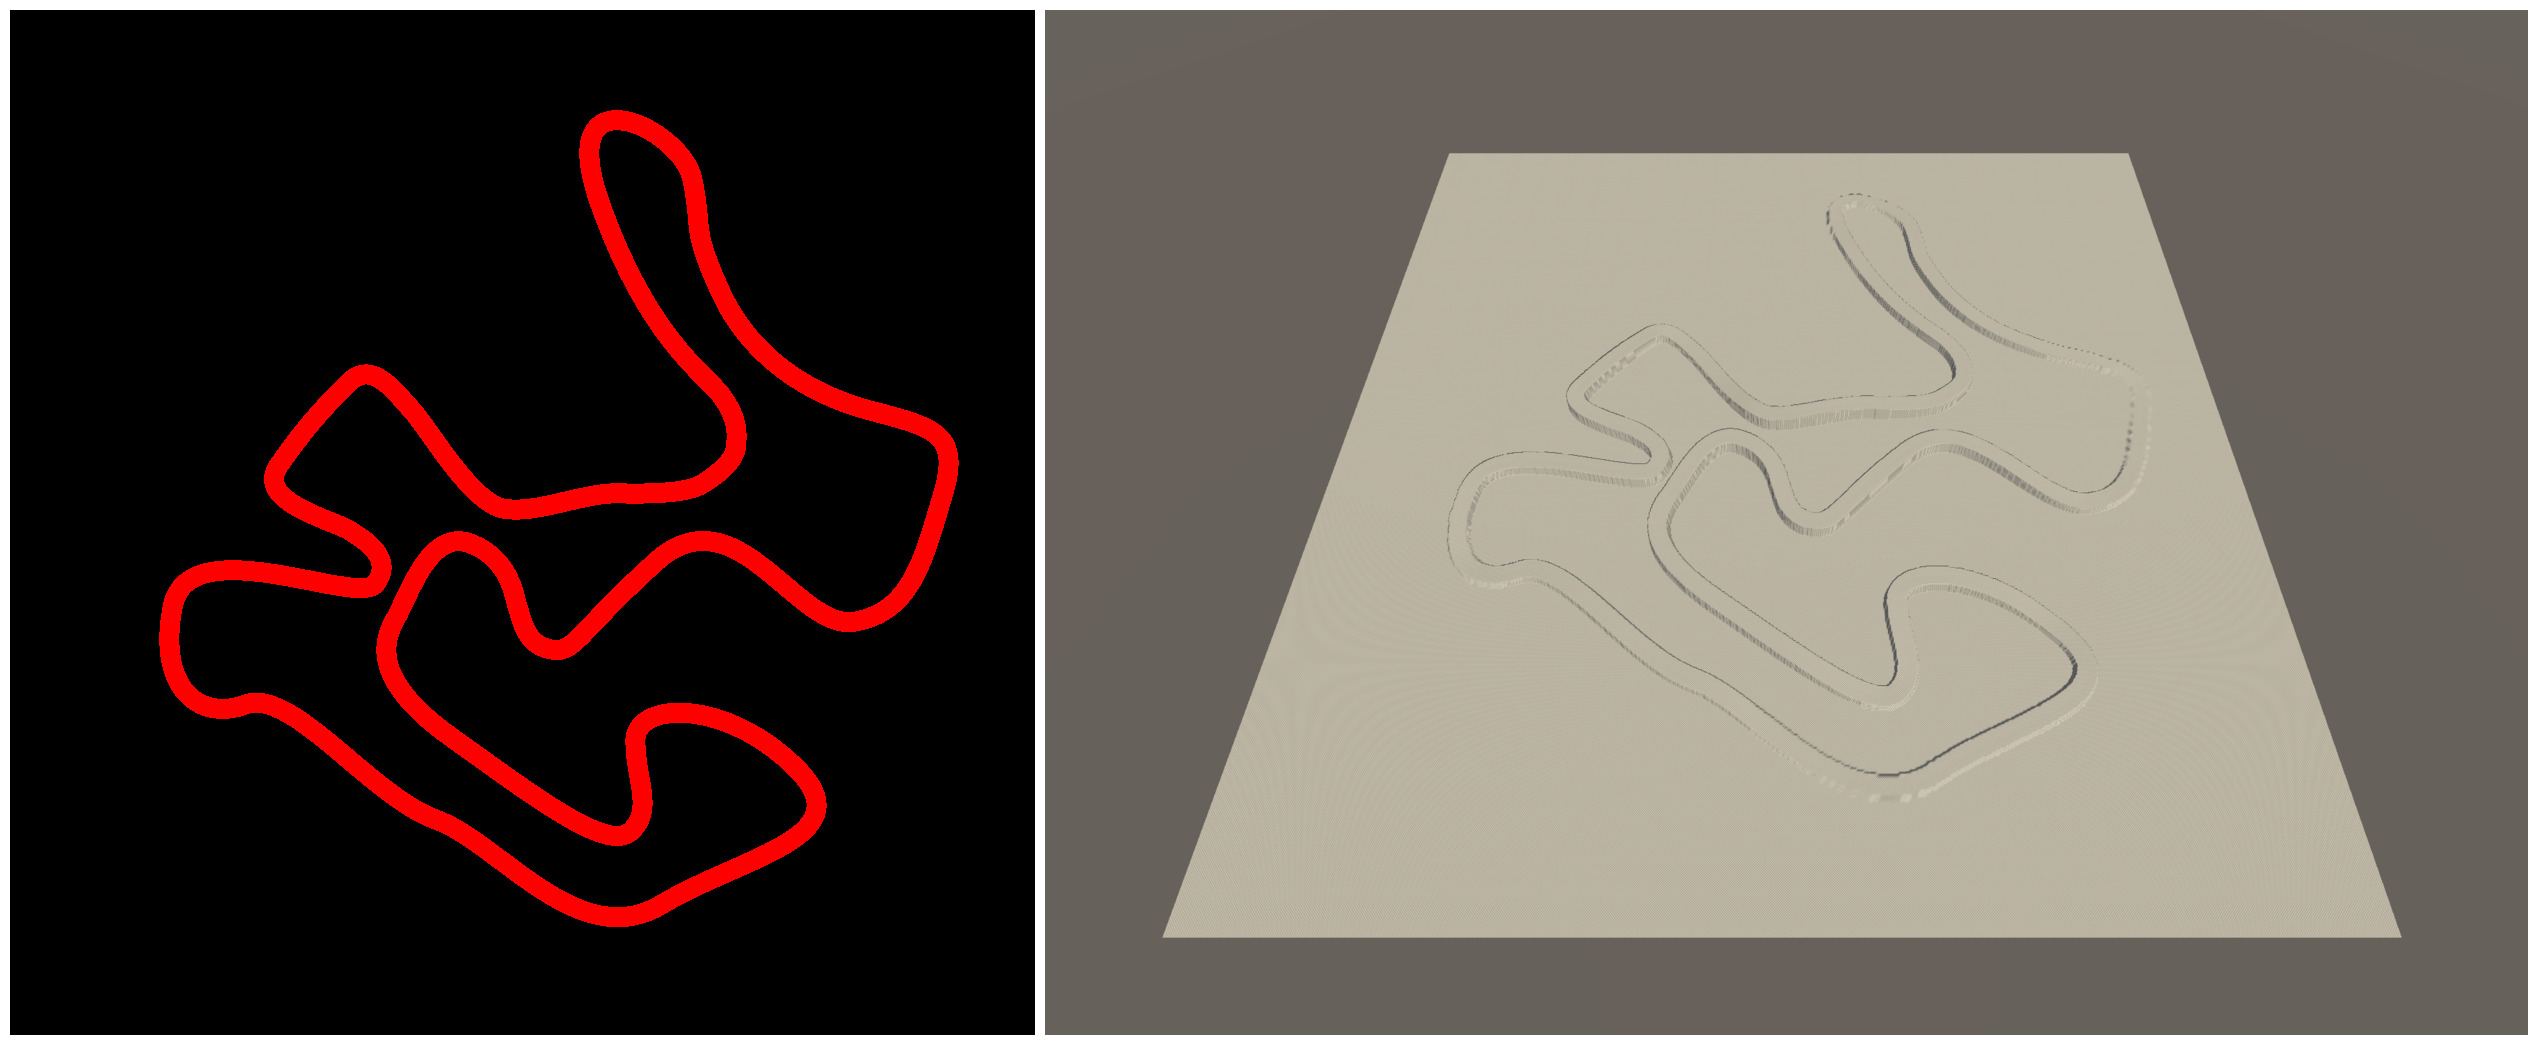
\includegraphics[width=1.0\textwidth]{img/iga_images/basis_terrain.jpg}
    \caption{(Left) constraint mask drawing, mapping non-modifiable pixels. (Right) corresponding terrain to mask with predefined heights set.}
    \label{fig:iga_basis}
\end{figure}

\subsubsection{Genome Representation}

The genome representation is a fundamental design decision that determines how candidate solutions are encoded and evolved. Unlike \textcite{Walsh10}, whose approach uses fixed-length binary strings encoding five terrain parameters, our system employs a more flexible representation that reflects the compositional nature of our terrain generation pipeline.

Each terrain \textbf{genome} in our system consists of a variable-length sequence of terrain operations, where each operation carries its own parameters. This representation offers several advantages, for example: genomes can contain different numbers and types of operations, enabling evolution of both parameters and pipeline structure. It also allows new operation types to be added without restructuring the representation. Intuitively, the genome directly corresponds to the applied operations, giving a more clear understanding of an individual candidate.

A typical genome in our system might contain operations such as:
\begin{verbatim}
Terrain Genome Operations: 
[
    VoronoiGenerator { PeakCount: 8, FallRate: 1.5, ... },
    PerlinNoiseGenerator { Frequency: 0.005, Octaves: 6, ... },
    DistanceBasedHeightScaler { MaxScaleFactor: 0.6, ... },
    EnhancedDistanceSmoother { Iterations: 40, ... },
    ThermalErosion { Iterations: 50, Threshold: 0.0015, ... }
]
\end{verbatim}

This representation captures both the operations to apply and their respective parameters, providing a rich space for evolutionary exploration.

\subsubsection{Population Initialisation and Evolution}

Our IGA system maintains a population of terrain genomes presented to users for evaluation, following the interactive evolution principles outlined in Section \ref{interactive_genetic_algorithms}. 

The initial population generation employs extensive domain knowledge to create intelligent starting points rather than purely random initialisation. Our smart initialisation system incorporates deep understanding of effective terrain generation sequences, ensuring that genomes follow natural progression patterns that respect both algorithmic dependencies and aesthetic principles.

\subsubsection{Smart Initialisation Heuristics}

Our system implements several domain-specific heuristics based on our understanding of successful terrain generation patterns:

\textbf{Operation Sequencing}: Every genome begins with a terrain generator (Perlin noise, Voronoi, or midpoint displacement) to establish base terrain features. This foundation is followed by height adjustment operations that scale terrain relative to constraint boundaries, ensuring smooth integration with fixed areas. Smoothing operations are strategically placed after major terrain modifications to create natural transitions. Finally, optional erosion and texture operations add surface detail and geological realism.

\textbf{Parameter Ranges}: Rather than using uniform random distributions, our initialisation biases parameters toward ranges that consistently produce visually appealing terrain. 

\textbf{Constraint-Aware Operations}: The system prioritises operations that work effectively with our distance-based constraint handling. Distance-based height scalers and enhanced distance smoothers appear in most genomes, as these operations directly address the boundary problem central to our approach. This ensures that evolved terrains naturally integrate with fixed height areas.

\textbf{Probabilistic Enhancement}: Certain beneficial operations are added probabilistically during initialisation. Erosion operations (50\% probability) add geological realism, while texture operations (50\% probability) provide surface detail. This probabilistic approach creates population diversity while maintaining fundamental genome quality.

This sequence demonstrates the logical progression from terrain generation through constraint integration to final refinement.

We also include a visual representation of initial individuals. For example, Figure \ref{fig:iga_initial} of our user-interface window (this is based on the terrain seen in Fig. \ref{fig:iga_basis}) shows the initial population generated. We can see the terrains are not that visually coherent in this generation, but it is a good start thanks to our heuristics, especially compared to random initialisation of operations.

\begin{figure}[ht]
    \centering
    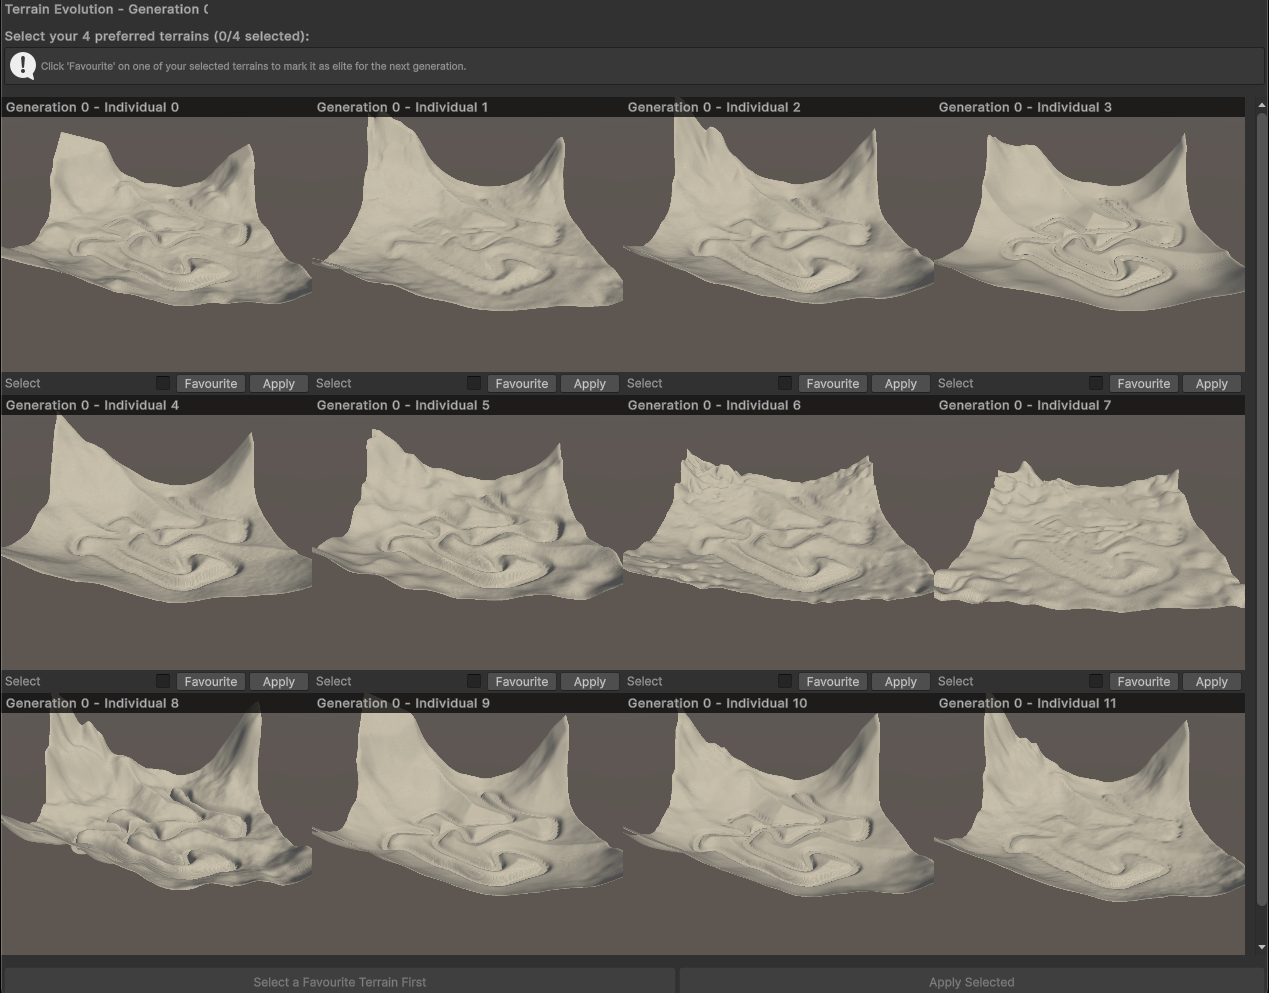
\includegraphics[width=1.0\textwidth]{img/iga_images/initial_gen.png}
    \caption{The Interactive Evolution interface showing an initial population of the terrain variants, each generated using different combinations of operations and parameters. These are all for the terrain from figure \ref{fig:iga_basis}}
    \label{fig:iga_initial}
\end{figure}

We will be using the following parameters for our example, which we chose to show a normal use case of the IGA: 

\begin{itemize}
    \item Population size -- 12;
    \item Selection count -- 4;
    \item Mutation rate -- 0.5;
    \item Crossover rate -- 0.8.
\end{itemize}

\subsubsection{Interactive Selection and Fitness Evaluation}

The selection mechanism in our IGA differs \textit{fundamentally} from traditional genetic algorithms. Rather than using a mathematical fitness function, \textbf{users} evaluate terrains \textbf{visually}, selecting those that best represent their aesthetic goals. This makes the process very subjective, as the final terrain will be heavily influenced by what the user deems a good candidate. This captures design intentions that would be difficult to encode algorithmically.

Our selection interface allows users to select multiple terrains that exhibit desirable characteristics, mark one terrain as a "favourite" for \textbf{elitist preservation}, apply any terrain directly to see it at full resolution, and continue evolution. The multi-selection approach provides rich feedback, allowing users to indicate different appealing aspects across multiple terrains.

This process is demonstrated in Figure \ref{fig:iga_selection} below, representing the selection interface window of our application:

\begin{figure}[h!]
    \centering
    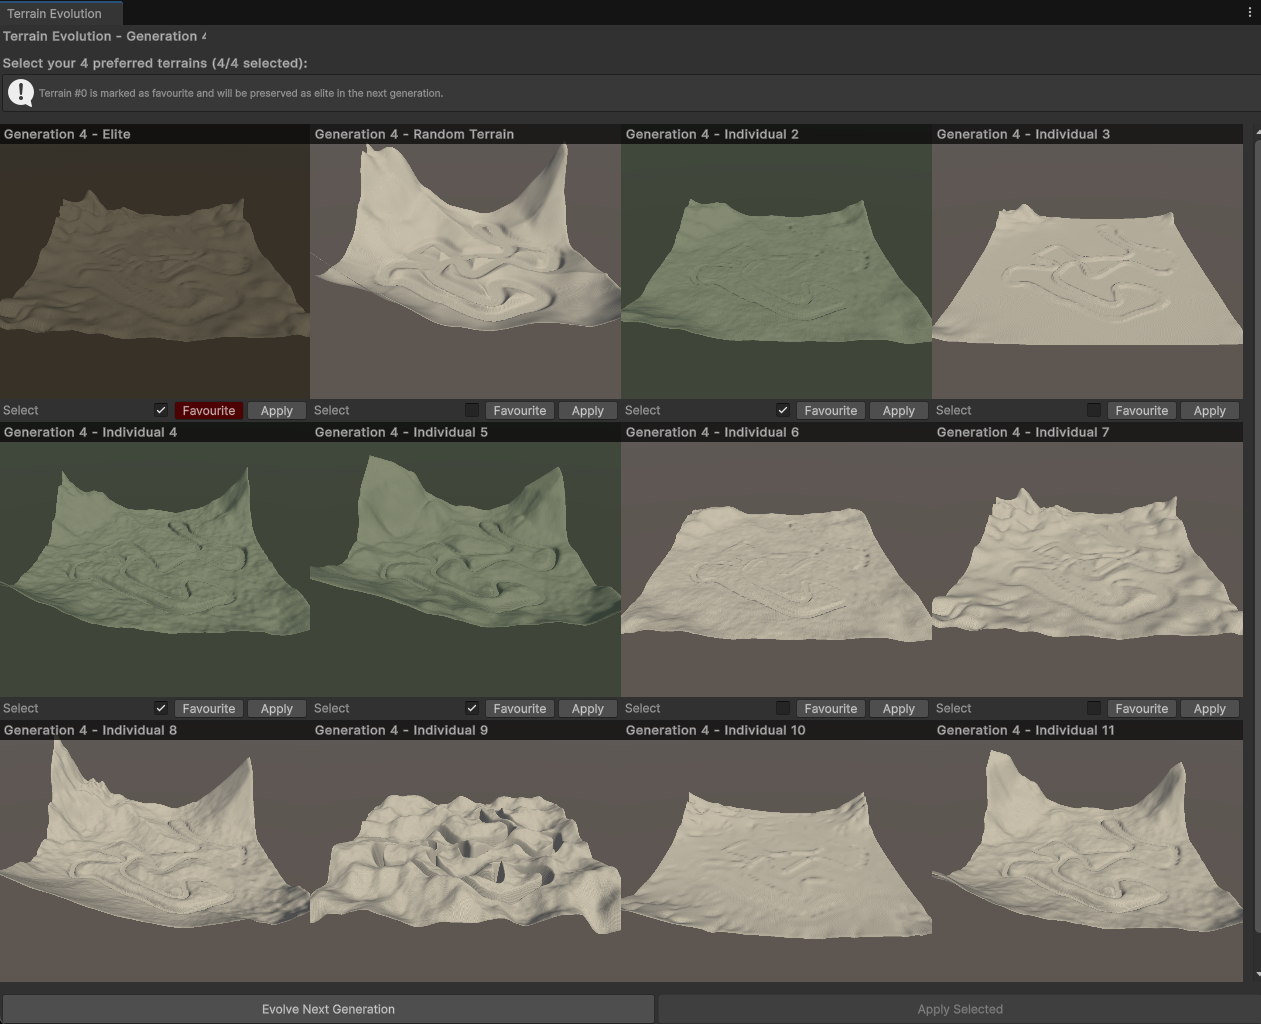
\includegraphics[width=1.0\textwidth]{img/iga_images/selection_window.png}
    \caption{The selection interface showing four selected terrains (green) with one marked as favourite (red) for elitist preservation in the next generation. This is the result after four generations.}
    \label{fig:iga_selection}
\end{figure}

The inclusion of an explicit ``favourite'' mechanism implements elitism, ensuring the best solution from the user's perspective is preserved across generations. This addresses a common problem in genetic algorithms where promising solutions can be lost through genetic operations.

\subsubsection{Genetic Operations}

Our genetic operations are adapted to work with our representation of a terrain genome.

\textbf{Crossover} operates at the operation level. Given two parent genomes, we select random crossover points in each parent, take operations before the crossover point from the first parent, and append operations after the crossover point from the second parent. 

\textbf{Mutation} Our mutation operators extend beyond random parameter modification to implement domain-aware genetic variations:
\begin{enumerate}
    \item [-] Structural Mutations: Rather than randomly altering existing operations, our system adds new operations at strategic locations. Height-scaling mutations insert multiple distance-based height scalers at different pipeline stages, creating graduated height transitions. Extreme smoothing mutations add intensive smoothing sequences to address particularly challenging constraint boundaries.
    \item [-] Texture Mutations: These operations add fine-scale detail through low-amplitude noise generators followed by appropriate smoothing. The system automatically adjusts parameters to ensure texture detail does not interfere with constraint boundaries.
    \item [-] To prevent genome bloat, removal mutations eliminate 3-6 operations randomly, allowing successful core operations to dominate the pipeline. This balances genetic diversity with computational efficiency.
\end{enumerate}

Below we present Figure \ref{fig:final_gen} that demonstrates the evolutionary progress of terrain variants over generations:

\begin{figure}[h!]
    \centering
    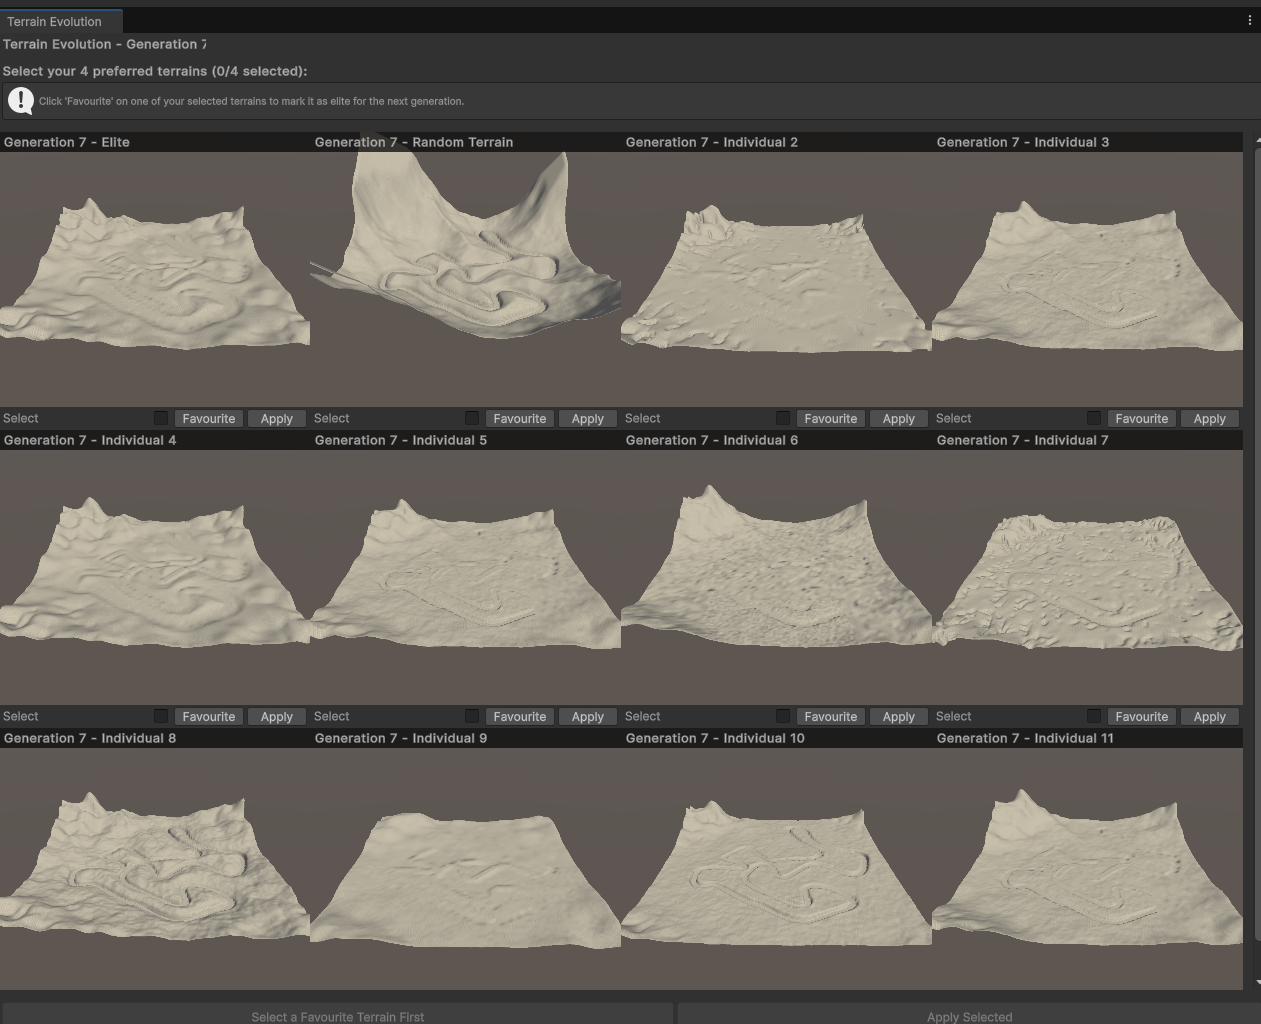
\includegraphics[width=1.0\textwidth]{img/iga_images/final_gen.png}
    \caption{Evolution progress showing terrain variants after multiple generations, demonstrating convergence toward user preferences to flatter terrains in this example, while maintaining some diversity.}
    \label{fig:final_gen}
\end{figure}

We also include Figure \ref{fig:iga_results_flat} which is the \textbf{elite} terrain taken from Fig. \ref{fig:final_gen} (top left). This demonstrates more clearly how well our IGA approach works.

\begin{figure}[h!]
    \centering
    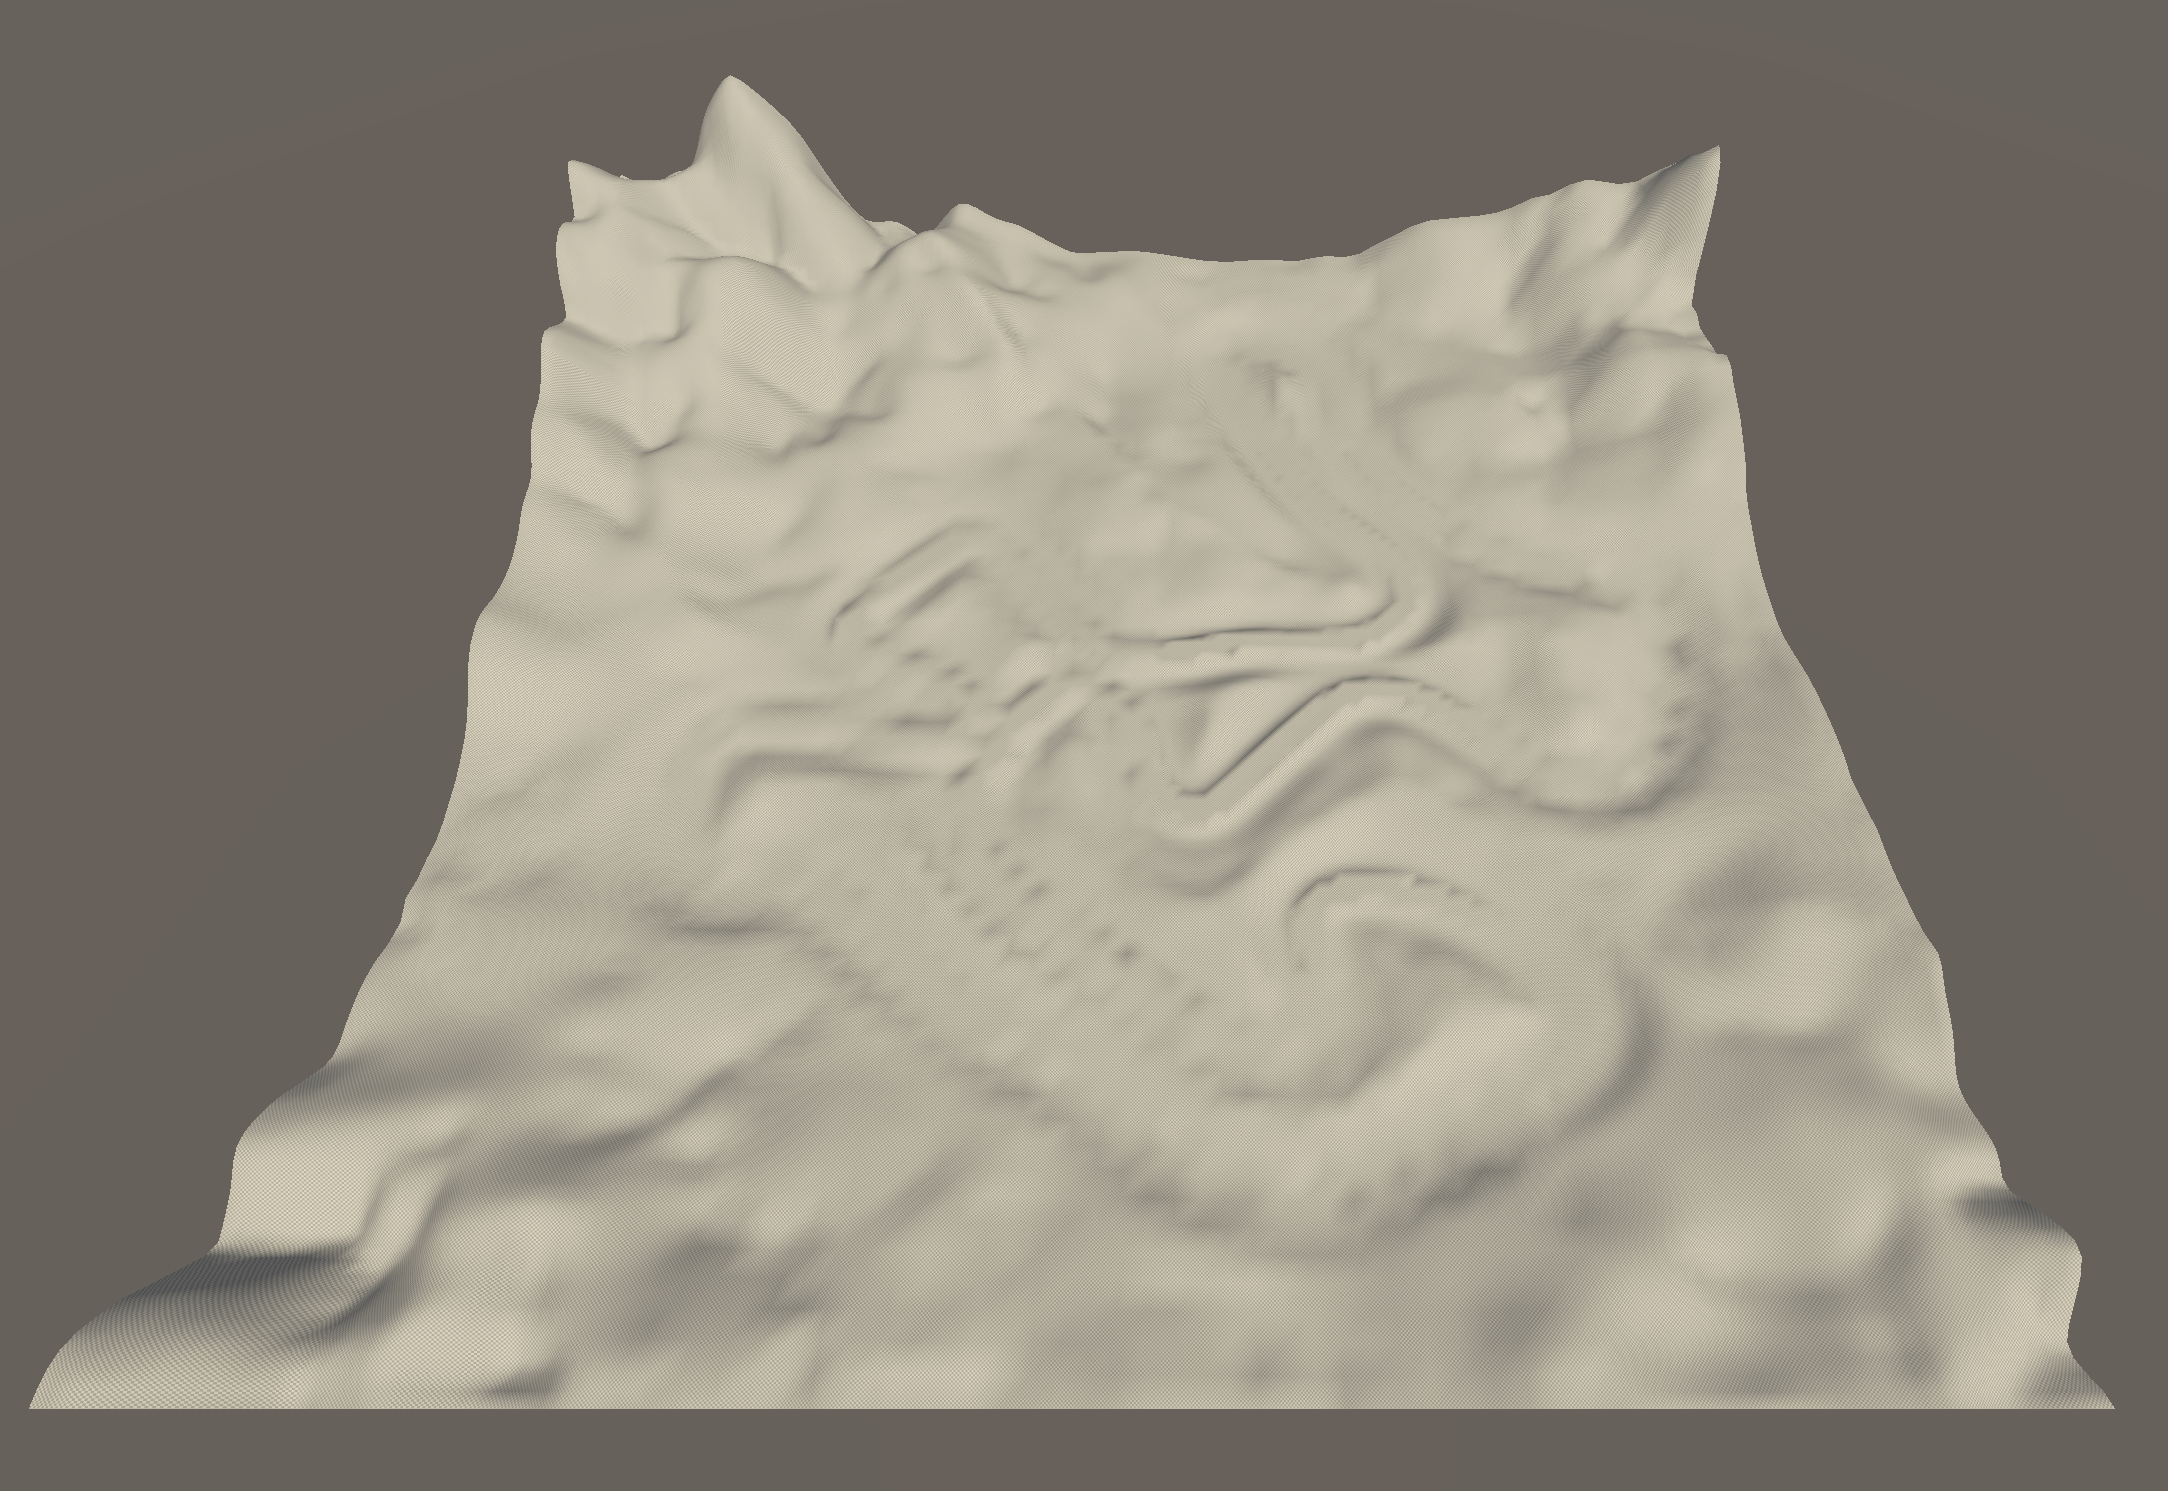
\includegraphics[width=1.0\textwidth]{img/iga_images/gen_7_result.png}
    \caption{Final terrain example from the 7th generation in the above terrain evolution window \ref{fig:final_gen}. This is the elite terrain (seen in the top left of the evolution window) applied to the actual terrain. This was fully generated using the IGA, where the user had a preference to a flat, bumpy terrain around their constraint.}
    \label{fig:iga_results_flat}
\end{figure}

\section{Implementation and User Experience}

Our IGA implementation leverages Unity's editor capabilities to provide an integrated, responsive experience. The system generates quick previews by capturing the current terrain state, applying each genome's operations, rendering from a carefully chosen camera angle, and restoring the original terrain. 

The evolution process typically converges toward satisfactory results within 5-10 generations, though users can continue evolving indefinitely to explore alternative solutions. The system's ability to discover novel parameter combinations often surprises users, producing terrain configurations they would not have considered through manual tuning.

\section{Parameter Tuning and System Configuration}
\label{parameter_tuning}

While our IGA system provides intuitive parameter exploration through human-guided evolution, the effectiveness of the evolutionary process itself depends on careful configuration of the genetic algorithm parameters. The balance between exploration and exploitation, a fundamental consideration in evolutionary algorithms discussed in Section \ref{genetic_algorithms_fundamentals}, directly influences both the quality of results and user experience.

\subsection{Core IGA Parameters}

Our system exposes four primary parameters that control the evolutionary dynamics:

\textbf{Population Size} determines the number of terrain variants presented to users in each generation. We usually use a population size of 12 - 32, as this is a good balance between efficiency and diversity. 

\textbf{Selection Count} specifies how many individuals users choose as parents for the next generation. We typically recommend selecting 25-40\% of the population (3-6 individuals). Higher selection pressure (fewer selected individuals) accelerates convergence but risks premature convergence to local optima. Lower selection pressure (more selected individuals) maintains diversity longer but may slow progress toward user preferences.

\textbf{Crossover Rate} controls the probability that two parent genomes will exchange genetic material. Our default of 0.7 balances recombination benefits with parent preservation. Higher rates (0.8-0.9) encourage exploration of new parameter combinations but may disrupt successful genome structures. Lower rates (0.4-0.6) preserve parent characteristics more strongly but reduce the algorithm's ability to discover novel solutions.

\textbf{Mutation Rate} determines how frequently random modifications occur in offspring genomes. Unlike traditional genetic algorithms that use low mutation rates (0.01-0.05), our system usually employs higher values (0.5-0.8) to compensate for small population sizes. The domain-specific nature of our mutation operators, which add terrain-appropriate operations rather than random parameter changes, allows for more aggressive mutation while maintaining genome viability.

\section{Summary}

In this chapter, we have presented our specific implementation of Interactive Genetic Algorithm techniques for parameter optimisation in constrained procedural terrain generation. Building upon the theoretical foundation established in Section \ref{interactive_genetic_algorithms} and the pioneering work of \textcite{Walsh10}, we have developed a practical system that addresses the parameter space complexity challenges detailed in Section \ref{parameter_space_challenge}.

Our key technical contributions extend beyond the basic IGA framework presented in Chapter \ref{Chapter1}: a flexible, operation-based genome representation that captures both pipeline structure and parameters; constraint-aware genetic operations designed specifically for our distance-based terrain generation approach; domain-intelligent initialisation leveraging terrain generation knowledge for quality starting populations; enhanced selection mechanisms including elitist preservation through user-designated favourites; and seamless Unity integration providing rapid visual feedback for interactive evolution.

The IGA addresses the fundamental challenge identified in Section \ref{parameter_optimization}: the formalisation of subjective terrain quality in procedural generation systems. By leveraging human judgment directly within the evolutionary framework, we create a system that naturally adapts to individual preferences and design goals while navigating the complex parameter interactions inherent in constrained terrain generation.